\chapter{Introduction}
\label{chap:intro}
\minitoc
\section{Context}

Making sense of texts plays a vital role on the evolution of general artificial intelligence. Given the constantly-growing generation of textual data, there is the need of computational systems able to extract useful information from large quantities of textual collections, mainly to facilitate our day-to-day activities and, not less important, to find useful latent information hidden behind these large quantities of data. For example (see Figure \ref{fig:google_nlp}), Google, the search engine giant, is now able to conveniently answer short questions by analyzing textual knowledge bases, such as the English Wikipedia, in order to find the answer. Furthermore, Gmail, Google's electronic mail client, now  automatically identifies events, and sometimes their location and participants, from our personal emails and then adds  them to our online agendas. On the other hand, finding relations among concepts within a set of documents can be a rich source of knowledge. An example: using text mining techniques, in the biomedical domain,  facts can be linked across publications generating new hypotheses directly from the literature \cite{garten2010recent}. 

\begin{figure}[t]
\centering
	\begin{subfigure}[b]{0.55\textwidth}
	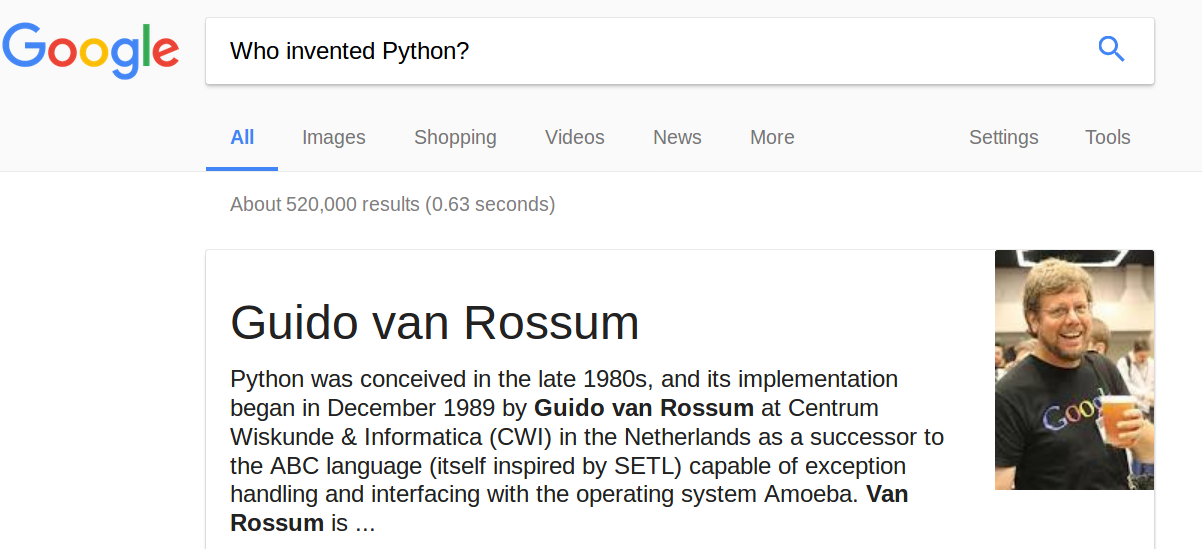
\includegraphics[width=1\linewidth]{./images/Chapitre1/guido_google.png}
	\caption{}
\end{subfigure}

	\begin{subfigure}[b]{0.55\textwidth}
	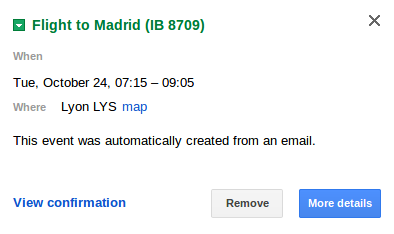
\includegraphics[width=1\linewidth]{./images/Chapitre1/calendar2.png}
	\caption{}
\end{subfigure}
\caption[foo]{(a) While searching \textit{Who invented Python?}, Google recongizes the simple question an directly gives us the answer from Wikipedia. (b) Gmail detects we received an email from an airline and parses it, finds the date, and automatically creates the corresponding event in our calendar.}	
\label{fig:google_nlp}
\end{figure}
%
Indeed, making computers learn,  via theories, algorithms and applications, is the general objective of artificial intelligence research \cite{Sugiyama2015}. Coming from this multi-disciplinary area, Natural Language Processing\footnote{And its more applied branch, text mining or text analysis. While it is sometimes argued that text mining deals with the structured data information extracted from text, I believe both terms considerably overlap nowadays. For ease of readability, in this dissertation we use both terms interchangeably, while preferring Natural Language Processing.} (NLP) is the domain that aims to make machines understand our language \cite{JurafskyM09} and thus making it possible to communicate with them in our own language. Specifically, speech and text, the latter being the focus of this work.

Although a challenging task, primarily given the ambiguity and dynamics of human language, NLP has developed rapidly \cite{ClarkBook2010} during the last two decades mainly due to the combination of three factors: 
\begin{itemize}
\item The  availability of \textbf{large quantities of freely-accessible textual data}: primarily enabled by the current Web technologies, we are today able to download with a single click the entire content of the English (or other languages) Wikipedia. In the same sense, we can also download thousands of gigabytes of Web crawled data. This information is used to derive knowledge about the text itself, as we will see in the rest of this dissertation. 
\item The \textbf{computational power} at our disposition: from consumer-based computers able to perform parallel computations with considerably large datasets; to on-demand distributed cloud platforms with high performance computing nodes. The latter may be from private providers, e.g., AWS Cloud Service\footnote{\url{https://aws.amazon.com/}}, Microsoft Azure\footnote{\url{https://azure.microsoft.com/en-us/}}, etc; or furnished by public organizations, such as France's Lyon 1 University\footnote{\url{https://p2chpd.univ-lyon1.fr/}} or the National Institute of Nuclear Physics computing centers\footnote{\url{https://cc.in2p3.fr/}}.

\item  The \textbf{large quantity of open-source text mining and data science analysis tools}. Luckily, it is becoming more common for NLP laboratories around the world to make their developments available to the general public, e.g, Stanford University CoreNLP\footnote{\url{https://stanfordnlp.github.io/CoreNLP/}}, Antwerp's University CLiPS Pattern\footnote{\url{http://www.clips.ua.ac.be/pattern}}.
% Paris 7's University Alpage Team Software\footnote{\url{https://www.rocq.inria.fr/alpage-wiki/tiki-index.php?page=Logiciels}}. 
Additionally, large Web companies, such as Facebook\footnote{\url{https://github.com/facebookresearch}} and Google\footnote{\url{https://github.com/google}}, frequently publish their research code and utilities. Lastly, communities of individuals develop libraries that grow to become essential building blocks of several applications and research in the domain. Notably, \texttt{scikit-learn}\footnote{\url{http://scikit-learn.org/}}, a popular data science library implementing several well-known machine learning algorithms. Regarding NLP specifically, two up-to-date libraries stand out:  \texttt{gensim}\footnote{\url{https://radimrehurek.com/gensim/}} and \texttt{spaCy}\footnote{\url{https://spacy.io/}}. These are, for the most part, cross-platform, high performance, optimized, well maintained, documented, and easily installable libraries.
% The former specializing on topic modeling and the latter on word's distributional representations.

\end{itemize} 
%
\begin{figure}
\centering
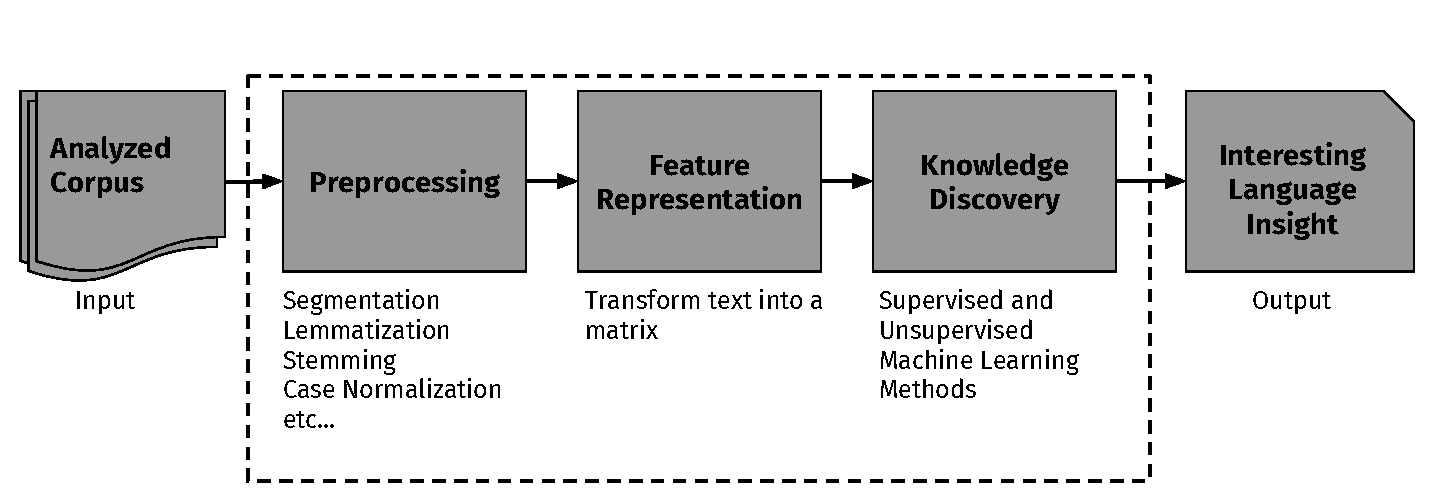
\includegraphics[width=1\linewidth]{./images/Chapitre1/nlp_flow.pdf}
\caption{Typical steps of Natural Language Processing applications.}
\label{fig:nlpflow}
\end{figure}
Solutions to NLP tasks generally follow three steps to achieve their respective goals \cite{mining12Book,JurafskyM09}. We can see in Figure \ref{fig:nlpflow}  the typical steps of a NLP system.  First, in \textbf{Preprocessing}, an input corpus is "normalized" so that it will be easier to treat it in the following steps. Secondly, in \textbf{Feature Representation}, numerous features are extracted from the preprocessed text. Thirdly, in \textbf{Knowledge Discovery},  a machine learning or rule-based (less common nowadays) technique is used to  learn a model able to provide an interesting insight within the existing data as well as on new future instances. The output of said system is usually the model or the language knowledge that reveals an interesting piece of information contained in the input corpus. 

Natural Language Processing is used today for several practical applications. From the elementary tasks that aim to extract linguistic features directly from the text, to more applied systems that employ said features to solve challenging problems. For example, as elementary tasks there is Part-of-Speech (PoS) tagging and Named Entity Recognition (NER). The former, PoS tagging, aims to determine a syntactic class (part of speech) for each word in a corpus \cite{JurafskyM09}. The latter, NER, determines if a proper noun is a place, a person, an organization or any other type of entity required by the final domain and application \cite{nadeau2007survey} . An intermediate task, Word Sense Induction and Disambiguation (WSI/WSD) determines and assigns the semantic meaning of a given word according to its context \cite{ClarkBook2010}.


More complex tasks that generally employ one or more of the aforementioned techniques in order to get more descriptive features from the text and thus get us closer to understand what is being discussed. As an example,  sentiment analysis which ultimate goal of this task is to determine the positiveness or negativeness (or neutrality) of an opinion expressed in a text \cite{liu2012survey}. In this case, it would be useful to know what words express a ``sentiment'': usually adjectives, categorized via PoS tagging; it would be informative to know what (or about who) we are talking about, with NER tagging; as well as the specific context of the words that are being used in the opinion, via WSI/WSD. 



\section{Challenges and Contributions}
There are several research challenges that arise from the choices taken in each one of the steps comprising the NLP system's flow (Figure \ref{fig:nlpflow}).
 In this thesis, we particularly focus on three challenges arising in both the Feature Representation and Knowledge Discovery phases. These challenges are: (1) modeling, extracting, and storing different types of linguistic features from raw text, (2) dealing with the sparsity inherent to text data features and also successfully combining them to get better representations, and (3)  finding	 relations  between words and then leveraging them in order to discover their latent relatedness and be able to solve NLP tasks.

%\begin{itemize}
% \item \textbf{Feature Representation:}
%	 \begin{enumerate}
%	 \item Modeling, extracting, and storing different types of linguistic features from raw text. 
%	 \item Dealing with the sparsity inherent to text data while successfully combining the different available text features.
%	
%	 \end{enumerate}
% \item \textbf{Knowledge Discovery:}
% 	\begin{enumerate}
% 	\item[3.] Finding relations  between words and then leveraging them in order to discover their latent relatedness and be able to solve NLP tasks.
%  	\end{enumerate}
%\end{itemize}


We propose three contributions, one in terms of theoretical modelisation and two in terms of NLP applications. Specifically, the contributions that we propose in this work are the following:
\begin{itemize}
\item a hypergraph network-based model to hold and combine heterogeneous linguistic data %as well as a tool to extract said data from unstructured text.
\item a network-based algorithm to discover semantic relatedness between linked words
\item a method to combine heterogeneous representations while at the same time alleviating the sparsity problem common while dealing with text features.
\end{itemize}
These contributions are tested and evaluated using two different NLP semantic tasks: Word Sense Induction and Disambiguation and Named Entity Recognition. We chose these two tasks as they are semantic problems directly benefited by methods  that are able to determine the relatedness among words, which is the case of the techniques we propose. Not less important, we attack these tasks as they are central building blocks of more intricate text analysis systems. Our propositions are built using open source tools and trained/tested using freely accessible corpora. We aim to make our software implementations are  to multi-threaded CPU computers when applicable.


\subsection{Modeling linguistic features}
\paragraph{Challenge}
Representing unstructured text within a model that describes textual units and their corresponding features is a critical step within a NLP process. Textual units -- either words, sentences, paragraphs, documents, etc -- need to be represented by some kind of model that will allow for numerical analyses to be applied. Usually, textual units are represented in a vectorial space, where each dimension represents a feature; or in a graph-like structure, where features link units together. Concerning the features themselves, their selection is often an empirical process determined  by the final goal of the NLP process at hand. Nonetheless,  we have access to several types of linguistic features, each one representing the text from different points of view.  Furthermore, texts usually containing large vocabularies involves the need of an efficient way of storing a corpus and its features. These possibilities entail the following research questions: \textbf{what type of model can we employ to represent a corpus through a set of heterogeneous features, extracted from itself, while keeping record of the relationships between textual units?} \textbf{How can we organize and store this model as simply and efficiently possible?} Answering these questions would allow us to  properly design and build a linguistic resource containing heterogeneous descriptions of the textual units\footnote{In this work we focus on words. As such, the rest of this dissertation deals with the representation of words.} adapted to solve NLP tasks.


\paragraph{Contribution}
We propose a linguistic resource in the form of an heterogeneous language network to be used as a first essential data model to solve Natural Language Processing tasks. 
During the last decade, graphs have been used to model textual data given its ability to naturally represent the dynamics and structured of text.

The originality of our work consists in taking into account different types of features, e.g., lexical, syntactical, and orthographic information; and unifying them under a single hypergraph structure. An hypergraph differs from a graph in that its edges may link several nodes together at the same time. This flexibility allows for simple and efficient access to the stored elements, either specific types of words or specific features. (revoir: advantages of hyperedges]
%
We use the proposed model as the starting point of our other two contributions: solving Word Sense Disambiguation and Induction and Named Entity Recognition. 

Lastly, as a proof of concept and in order to test the implementation practicality of our model, we process the English Wikipedia corpus and store its heterogeneous features under the form of the proposed model. We particularly focus onto the lexical and syntactical characteristics of words.

\subsection{Leveraging the network to find semantic relatedness}
\paragraph{Challenge}
Leveraging the structure within the proposed linguistic network is one of our main reasons to build such a graph-based language resource. This structure, namely the features linking words  together, originate groups or communities of related words within the network. In that sense, leveraging these latent communities is still today an open question in the domain of graph-based NLP. Particularly in the context of semantic NLP tasks, where determining the relation among words is of utmost importance, we rise the following questions: \textbf{what kind of communities exist within language networks?} \textbf{How can we find and employ them to solve NLP tasks?} Furthermore, assuming an heterogeneous network like the one we propose, \textbf{what are the quantitative and qualitative differences, both in terms of performance and results, between the different representations existing within the network?} Determining the structure inside a language network, as well as devising an algorithm to exploit it would allow us to better understand the role of communities in  graph-based approaches for NLP. Finally, getting a glimpse of the differences between each heterogeneous feature can help us to decide which is the most appropriate according to a NLP system objective. 


\paragraph{Contribution}
Linguistic networks are complex structures that may hold  heterogeneous entities and links together. Properly leveraging these structures has been indeed a popular area of research in the NLP literature. 

We propose a variant to a literature algorithm that solves word sens induction and disambiguation mainly by leveraging  the structure of a language network in. The assumption of the algorithm is that of the network having "real-world" characteristics, broadly, this means that there are several tight-knit groups of words within the structure. Nonetheless, contrary to the existent model, our proposition differs regarding the considerably lower number of parameters by adjusting them automatically according to the statistics of the concerned network. We also allow for more flexibility of the studied contexts of each word. Furthermore, we leverage the structure of our proposed linguistic model and go beyond the classic homogeneous cooccurrences by studying the effect of heterogeneous features on the quality of the senses induced by the system. Our experiments show the interest of our method by improving on the performance of similar methods and by being on the same ballpark of state-of-the-art methods. We also thoroughly analyze the characteristics of the results --the word senses-- according to the different types of  obtained by our system.

 This We  improve the overall performance compared to other similar graph-based techniques.

\subsection{Combining features and dealing with sparsity}
\paragraph{Challenge}

While the proposed linguistic network contain heterogeneous features, in our previous propositions we have exclusively employed them separately. Nonetheless, employing these different attributes on a single textual representation is equally useful in terms of solving NLP applications. A certain type of feature may indicate relations that are completely unknown in another representation space. Thus a certain type of features can complement another to improve the overall description of words.

Another challenge that arises when building large cooccurrence networks, such as ours, is data sparsity. Indeed, sparsity is one of the main characteristics of textual data. Natural language processing systems rely on accurate information being found within a corpus. However, it is hard to see all the possible word cooccurrences in an input corpus and thus a system trained from it is not able to apply the acquired knowledge when it encounters unseen words and their cooccurrences.


Towards addressing both challenges previously described we pose the following questions: \textbf{how to alleviate data sparsity on textual data?}  Concerning combining linguistic features, h\textbf{ow can we produce a single textual representation  that is able to leverage the complementarity among features?} Lastly, \textbf{what is the behavior of combining features against using them independently?} The answer to these questions may shed light into more robust NLP systems, able to cope with sparsity while leveraging at the same time useful information coming from different types features.


% We explore multimedia fusion techniques to complement the features hold by the netuwork. Specifically, we focus on solving named entity recognition and word sense induction and disambiguation by applying feature-combination methods that have already shown their efficiency in the multimedia analysis domain.  Our results show that the combination of textual features indeed improves the performance compared to single feature representations and trivial features concatenation. Even more, we experiment with background information from open text sources to further improve the performance of our models. Finally, we also present an analysis on the behavior of features according to different types of senses and entity classes.



\paragraph{Contribution}
%\newpage












%\section{Contributions}
Addressing the sparsity of textual data is not an easy task and often involves complex procedures and loss of information. To alleviate this issue, we propose the application of multimedia analysis fusion techniques to solve NLP semantic tasks. The fusion methods we employ comprise a set of methods to combine (or fuse) different types of features into a single unique representation. While combining attributes we also enrich them by leveraging the complementary information  they carry individually. Furthermore, we address the challenge of data sparsity by transferring unseen relations from one feature space to another, that is, we obtain a denser similarity space by joining together both feature spaces. The experiments we carry out, in word sense induction and disambiguation and named entity recognition, show the pertinence of our approach. Specifically, we try different fusion techniques as well as several fusion configurations to improve the tasks' performance compared with using representations independently. Additionally, we study to what extent each type of fusion employed affects the performance of the tasks we evaluate.



\begin{figure*}
\centering
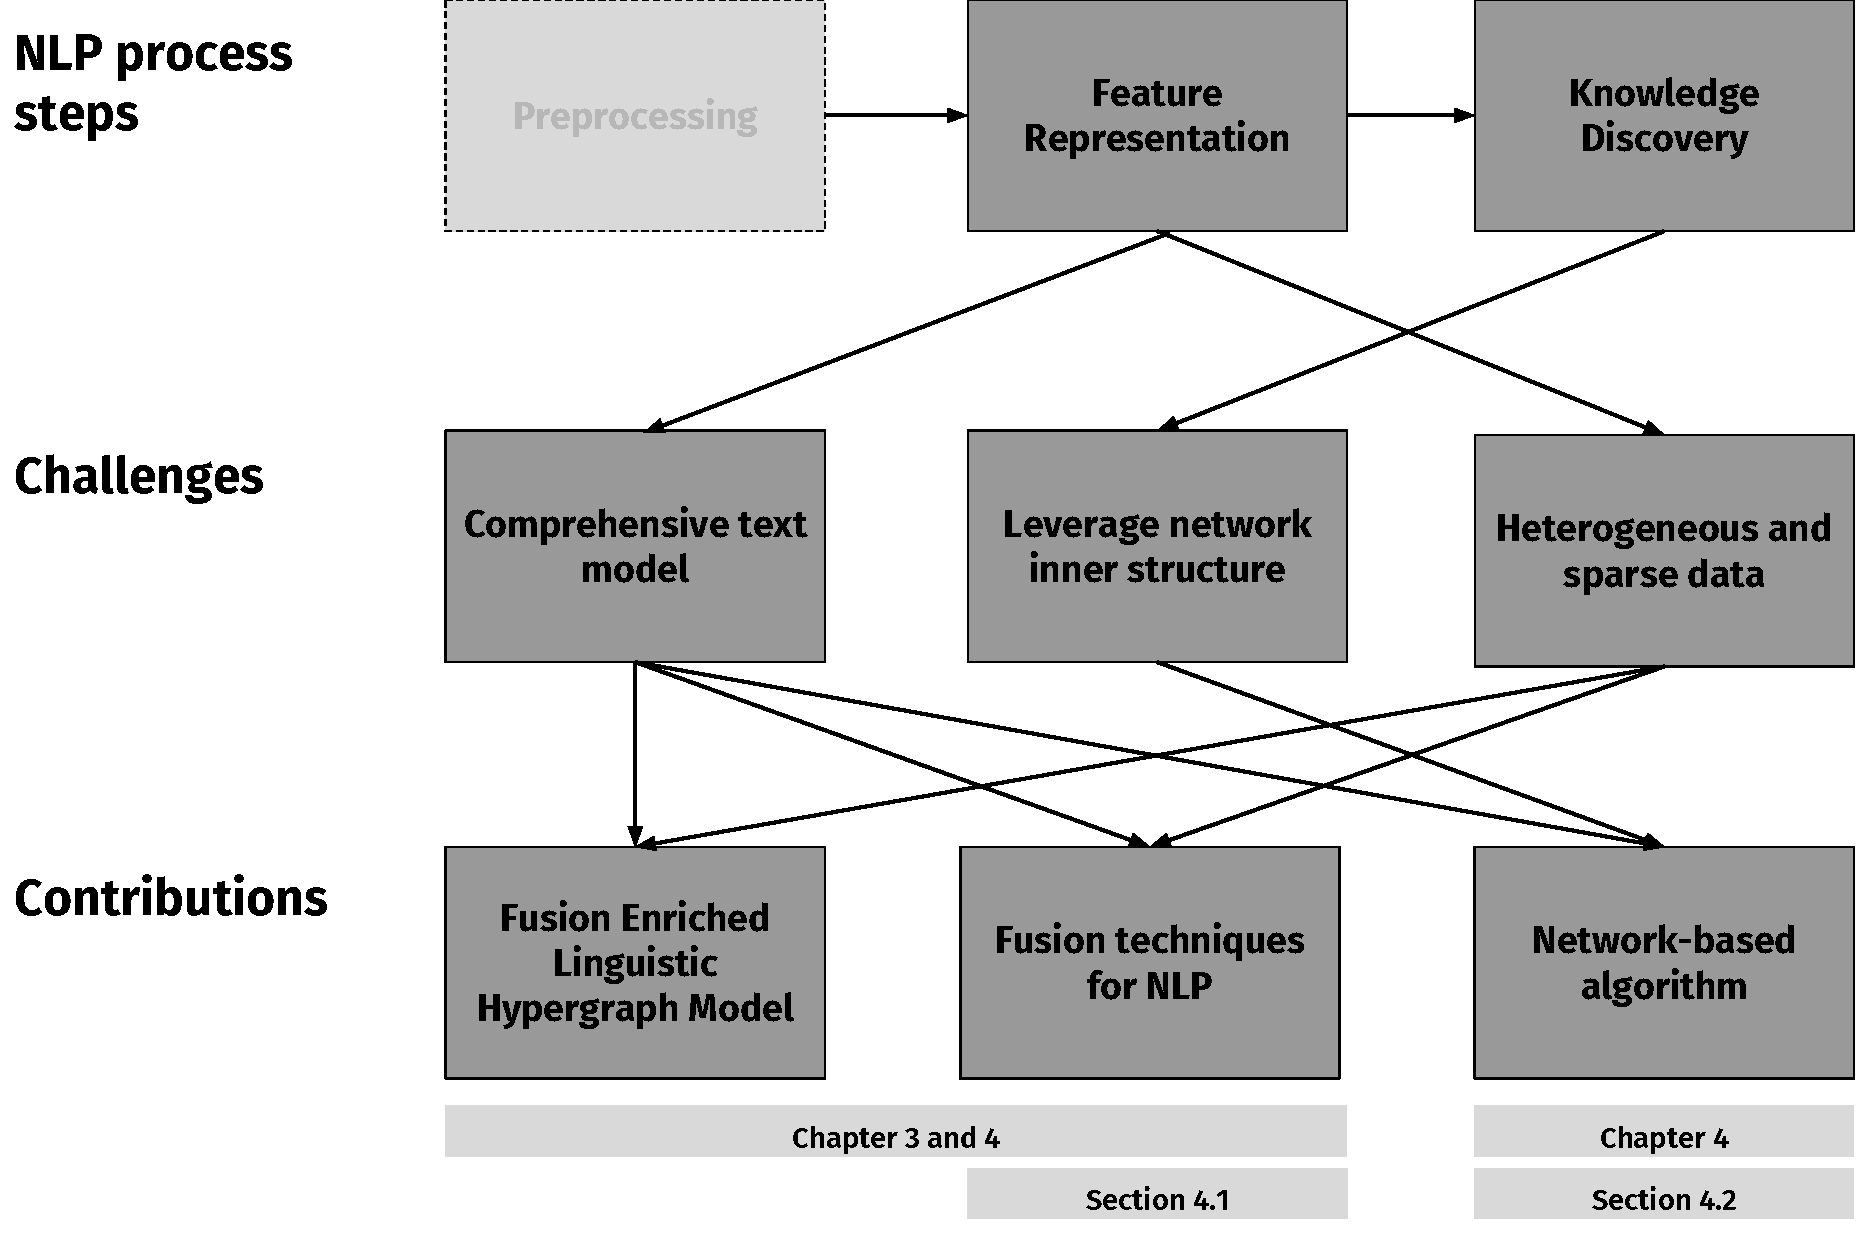
\includegraphics[width=1\linewidth]{./images/Chapitre1/challenges_contribs.pdf}
\caption{Block diagram of the NLP steps of interest, the challenges we address, and the contributions we propose.}
\label{fig:challenges_contribs}
\end{figure*}
\section{Structure of the Dissertation}

Figure \ref{fig:challenges_contribs} synthesizes the concerned NLP process-flow stages of this work (first line), the challenges that we aim to alleviate (second line), and their effect on the contributions we propose (third line). The remainder of this thesis is structured as follows:

\paragraph{Chapter \ref{chap:backgnd}} This chapter contains the theoretical background on the concepts discussed in this thesis. At the same time, we present the state of the art on the techniques that are relevant to our work. Specifically, we discuss the basics on text representation and how they are all related together by the distributional hypothesis. We then introduce the two main types of mathematical entities to manipulate text in a computer: vector-space models and graph-based models. Given our choice to work with graphs, we continue this path and introduce their basic concepts and move onto how graphs are employed to hold textual data as well as some prominent NLP applications in the literature. 
%Afterwards, we present how these features can be combined to improve the results of single-feature based solutions. 
Finally, we detail the machine learning methods we employ in certain as part of our methodology. 

\paragraph{Chapter \ref{chap:ling_net}} This As our first contribution, we present and define a novel structure to hold language information: the hypergraph linguistic model.  We discuss its characteristics and the intuitions behind its conception: the hypergraph choice,the role of nodes and edges, the type of features stored, the advantages it represents in terms of accessing and manipulating the data. 

This chapter describes the process of parsing and storing an English Wikipedia Syntactical Dump. We use open source tools on freely available data to generate a software that is able to extract lexical and syntactic data from a given corpus.We thus create and publicly release a syntactically annotated version of the English Wikipedia containing often-neglected information, stored in a format that facilitates its manipulation. 
\paragraph{Chapter \ref{chap:wsd}} In this chapter, we present an algorithm that exploits the structure of the network, i.e., the connections between nodes. Namely, we derive senses from a test corpus by finding related words connected to a single main node. We test the linguistic and lexical features and discuss about its qualities. Our results improve on the performance of similar propositions from the literature. We study the combination of features using multimedia fusion techniques in the next chapter.

We explore the application of multimedia fusion techniques using linguistic features to solve NLP tasks. Briefly, fusion techniques may consist on trivially concatenating feature columns or a combination that aims to transfer relatedness information from one representation to a second one. We experiment with these methods on three datasets for named entity recognition and one dataset for word sense induction and disambiguation. Indeed, we show that using certain configurations of fusion techniques can lead to improvements over single-feature and trivial-concatenation representation matrices. Furthermore, we explore the contribution from each representation kind to each sense and class in each task respectively.

\paragraph{Chapter \ref{chap:conclusions}} We conclude this dissertation and present possible avenues for future work.

